\section{Methodology}
\subsection{SeeSet V1 Dataset}
\label{sec:seeset}
To ensure a comprehensive and realistic evaluation of the atmospheric visibility problem, encompassing both ground-level and elevated altitude conditions, we introduce a novel framework incorporating multiple modalities. 
To overcome the limitations encountered in the previous studies and to include a broader range of real-world scenarios, we collect a novel aerial imagery dataset SeeSet v1. This dataset was carefully curated to incorporate dynamic views capturing ever-changing scenery, thereby encompassing both ground-based and aerial perspectives. 

In this section, we present first a detailed description of the data collection and labeling process (\ref{data_collection}). 
In \ref{modalities}, we present the extraction techniques used to generate the additional image modalities. 


\subsubsection{Dataset Collection Process}
\label{data_collection}

To generate our synthetic dataset, we utilize an FAA-approved flight simulator. This advanced simulator facilitates the controlled acquisition of images, showcasing diverse viewpoints and a range of visibility degradations. The process, as illustrated in Figure~\ref{fig:data_collection_process}, starts at ground-level altitude. We systematically increased visibility in incremental steps, extending up to 100 miles. Subsequently, when the visibility reaches the limit, we elevate the viewpoint's altitude and then reset the visibility to 0, continuing this procedure up to a maximum of 2000 feet AGL.


\begin{figure}[htbp]
\centerline{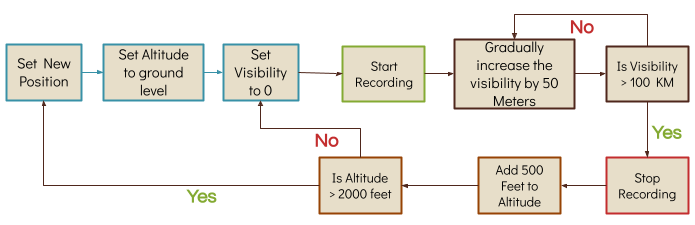
\includegraphics[width=250pt]{imgs/data_collection_pipeline.png}}
\caption{Dataset Collection Process}
\label{fig:data_collection_process}
\end{figure}
 

The collected images are automatically labeled into five discrete bins, each tailored to specific \href{https://www.faa.gov/air_traffic/publications/atpubs/aim_html/}{FAA requirements}. This categorization is based on visibility conditions and regulations relevant to both ground-based and aerial environments. The designated bins serve as the basis for the five labels utilized in training our DL models. 
We report the classes (bins) specifications and the corresponding counts in Table~\ref{tab:vis_img_count}.



\begin{figure*}
    \centering
    \subfigure[Bin 0]{
    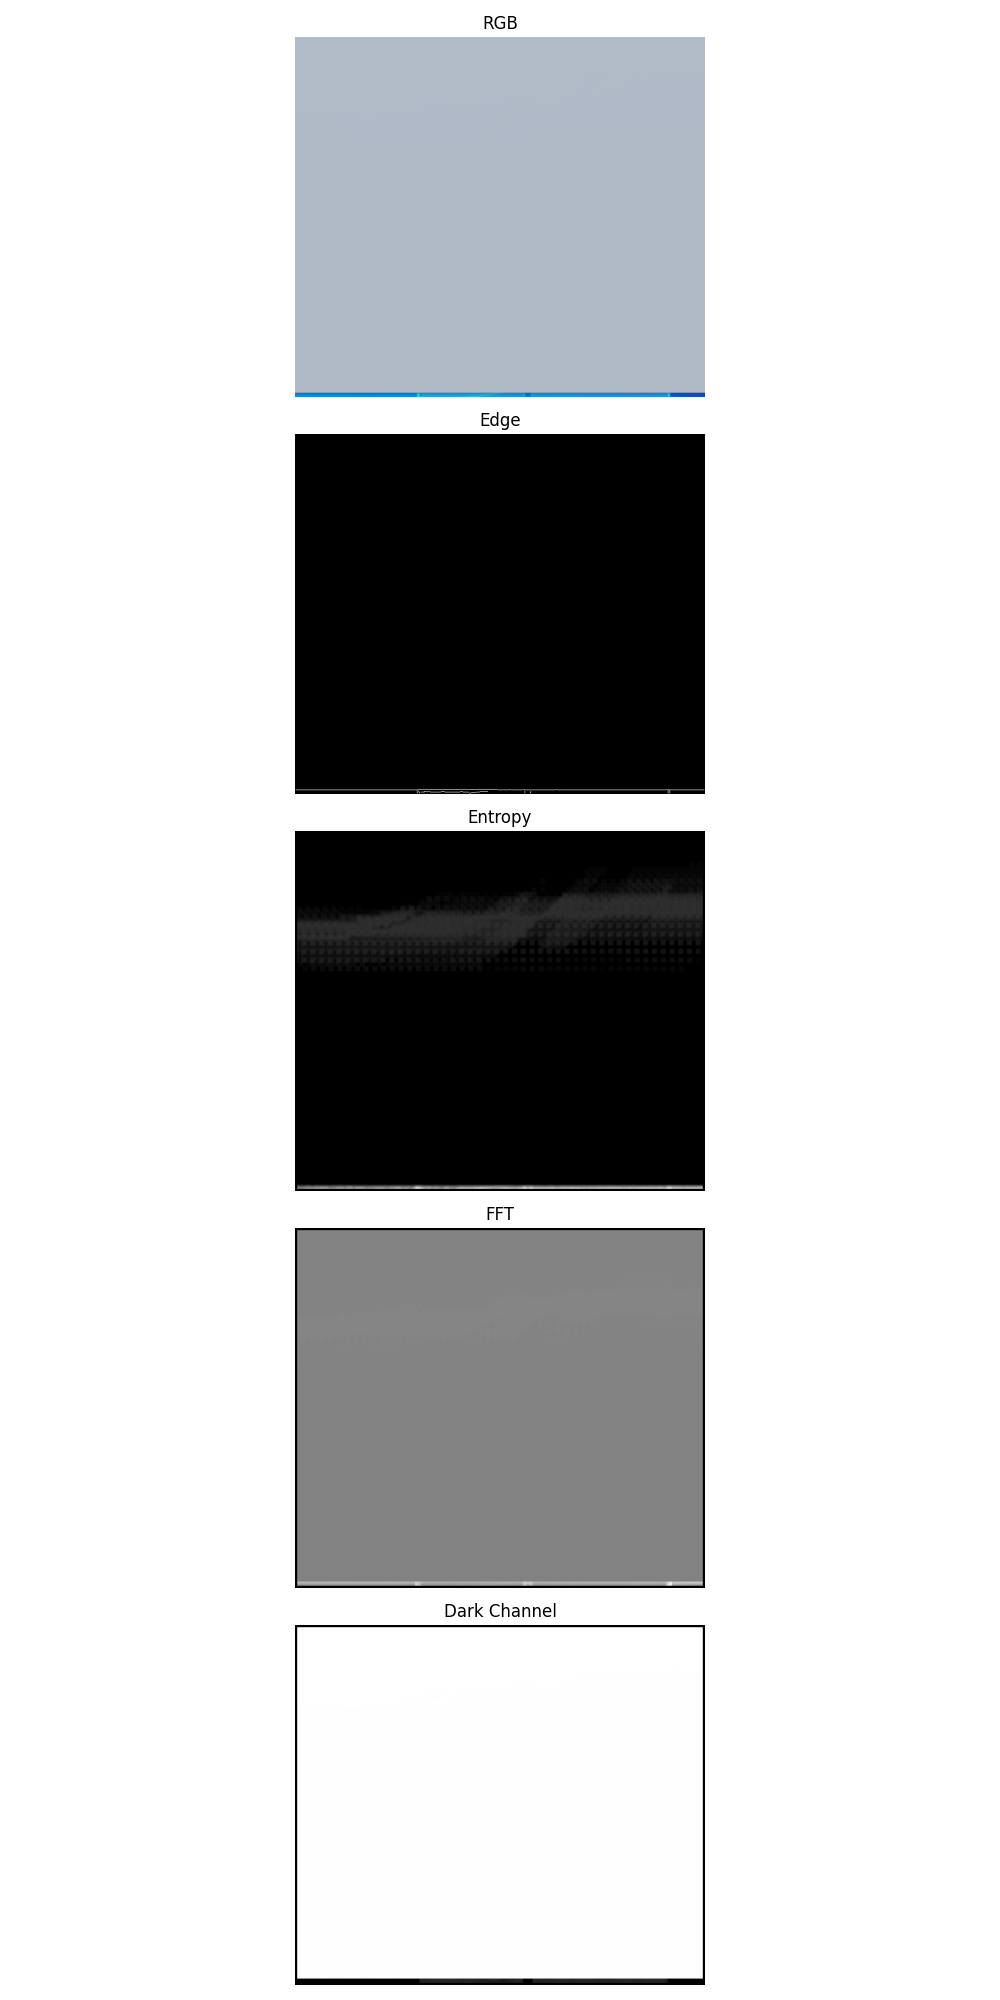
\includegraphics[width=0.14\textwidth, trim={7.5cm 0 7.5cm 0},clip]{imgs/examples/exp_0_featuresMiles_0.12427454732996136_featuresM_200_features.png}
    \label{subfig:bin0}
    }
    \subfigure[Bin 1]{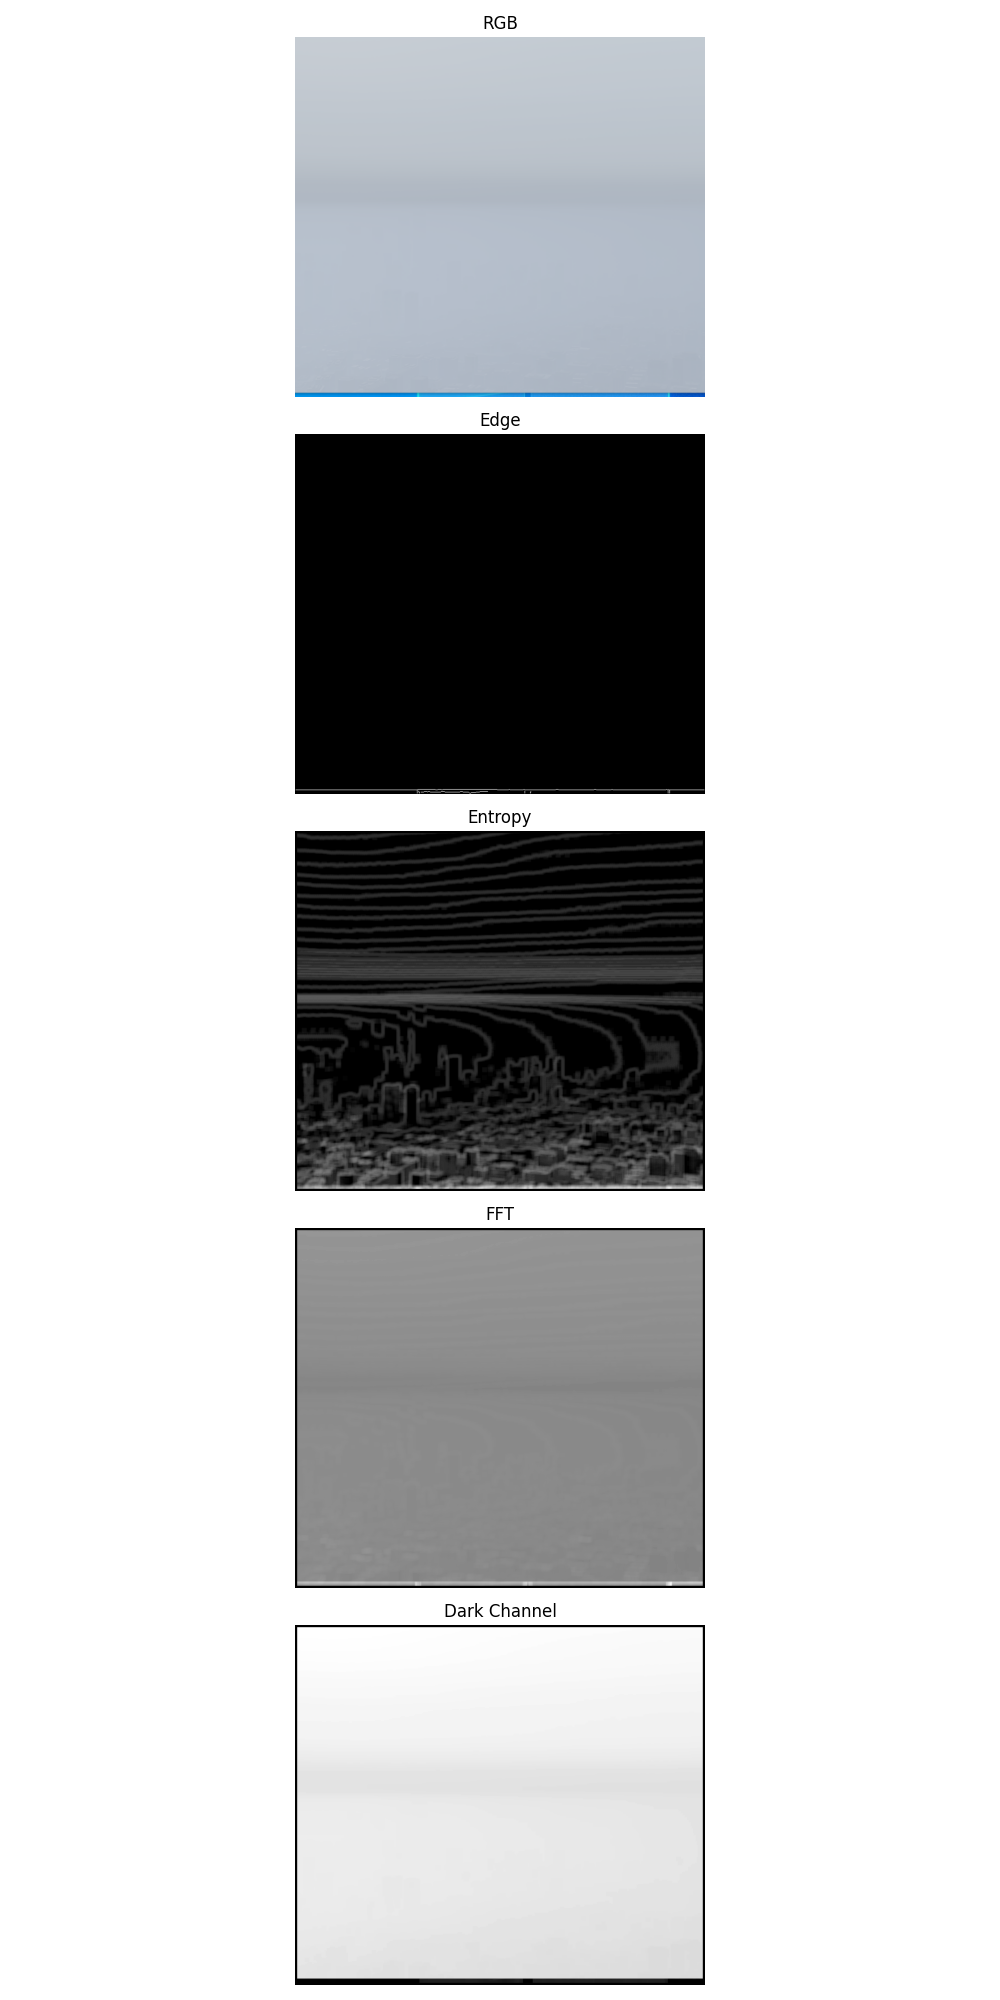
\includegraphics[width=0.14\textwidth, trim={7.5cm 0 7.5cm 0},clip]{imgs/examples/exp_0_featuresMiles_0.9320591049747102_featuresM_1500_features.png}
    \label{subfig:bin1}
    }
    \subfigure[ Bin 2]{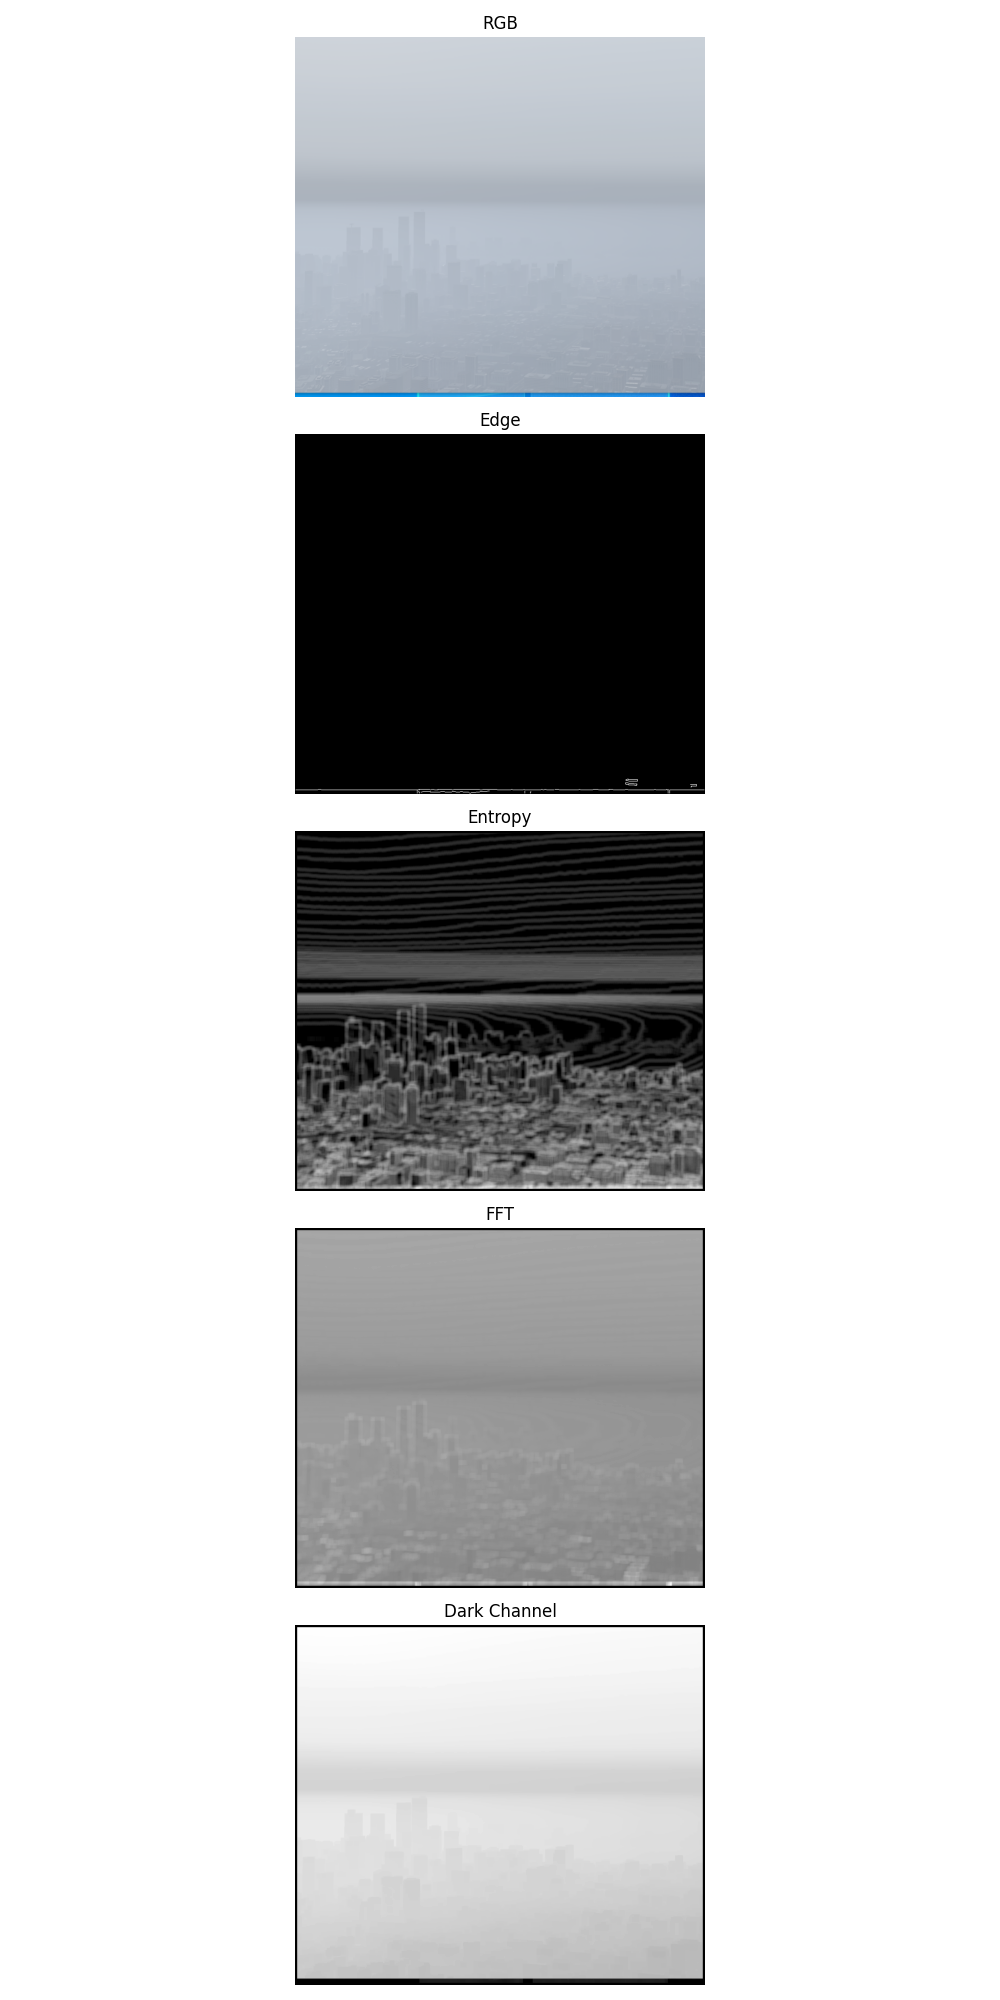
\includegraphics[width=0.14\textwidth, trim={7.5cm 0 7.5cm 0},clip]{imgs/examples/exp_0_featuresMiles_1.8951868467819106_featuresM_3050_features.png}
    \label{subfig:bin2}
    }
    \subfigure[Bin 3]{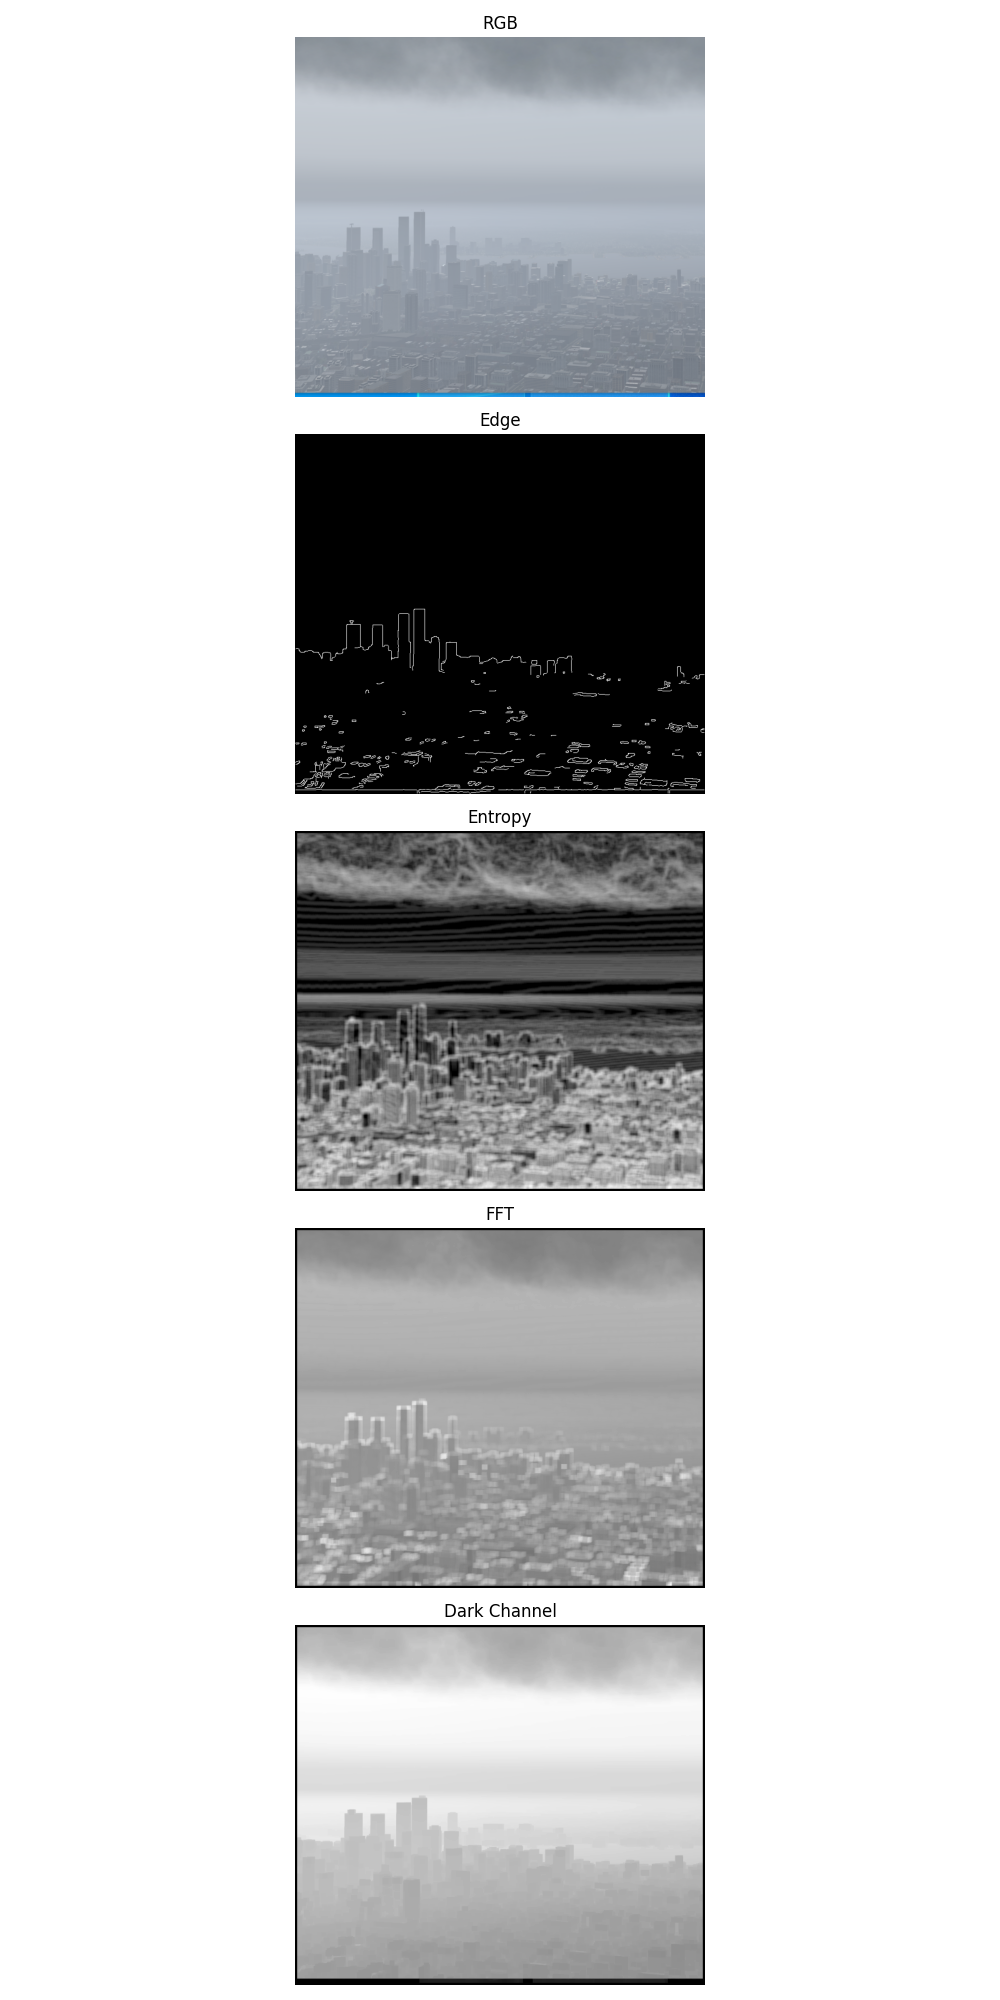
\includegraphics[width=0.14\textwidth, trim={7.5cm 0 7.5cm 0},clip]{imgs/examples/exp_0_featuresMiles_4.038922788223744_featuresM_6500_features.png}
    \label{subfig:bin3}
    }
    \subfigure[Bin 4]{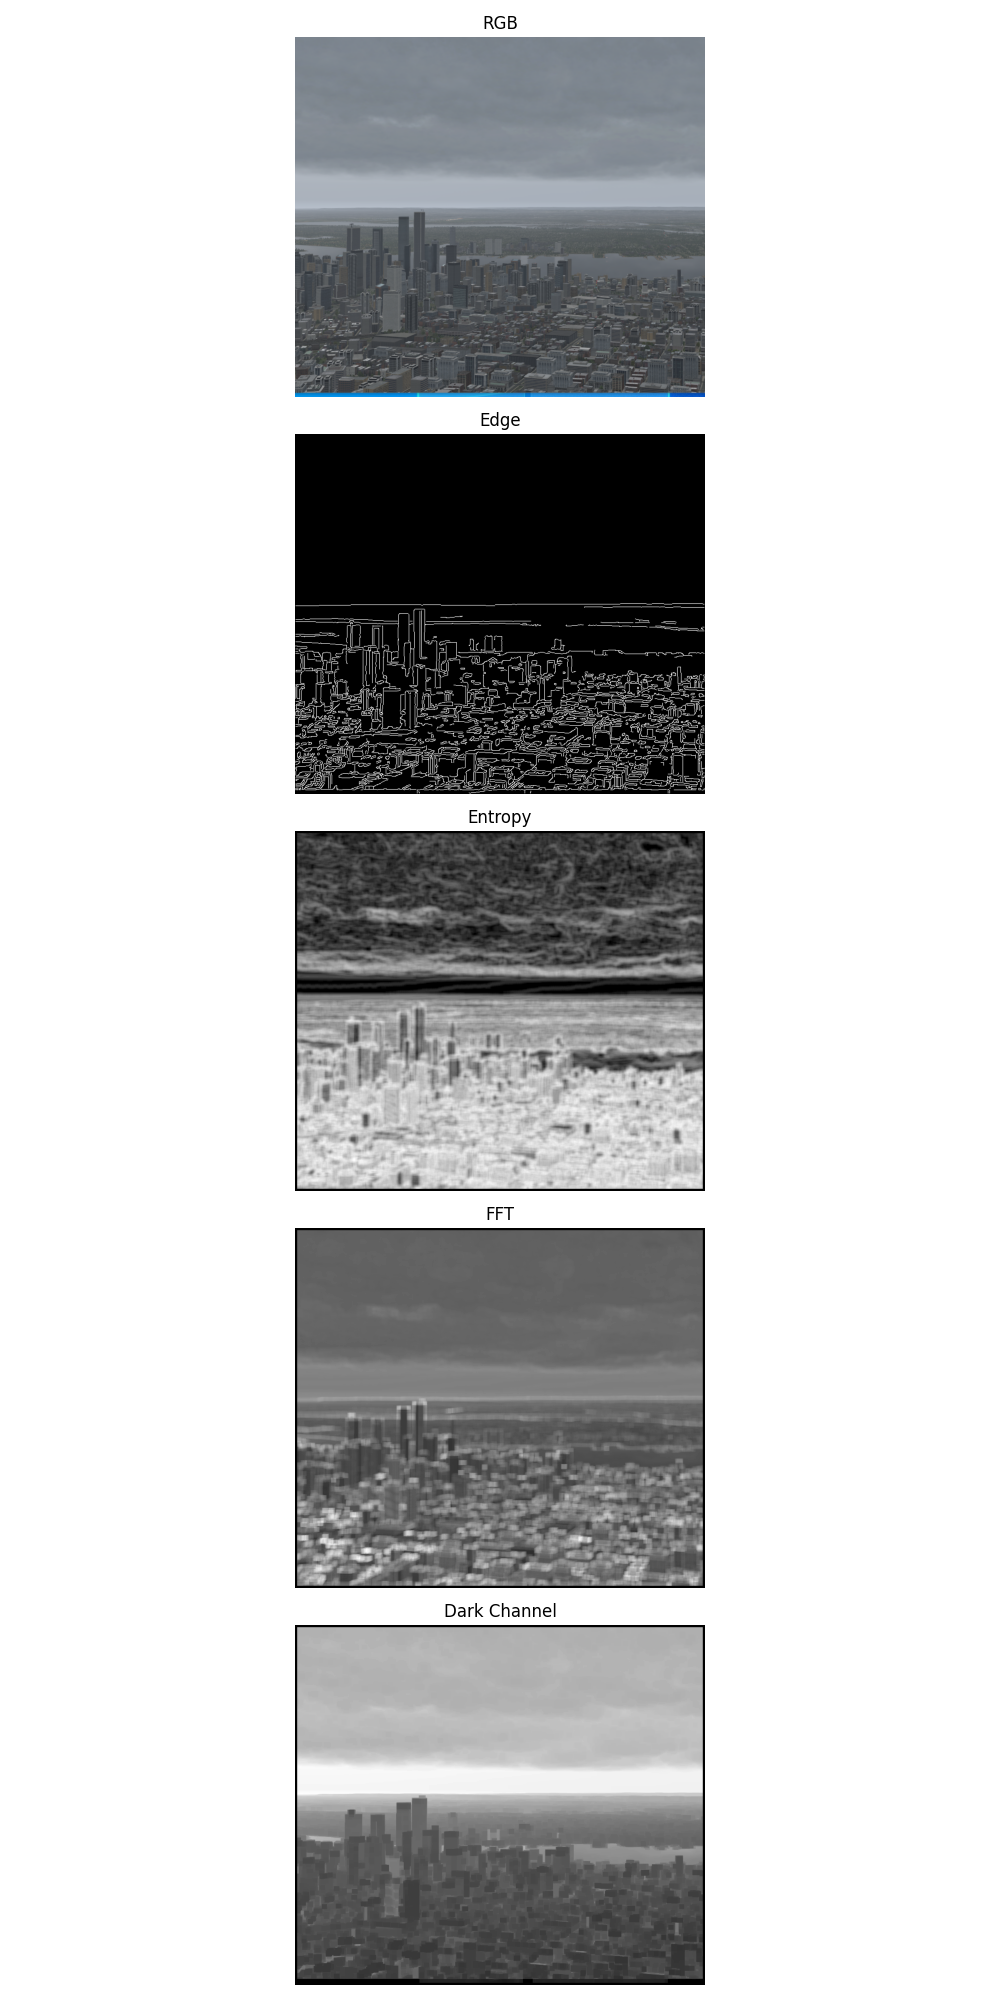
\includegraphics[width=0.14\textwidth, trim={7.5cm 0 7.5cm 0},clip]{imgs/examples/exp_0_featuresMiles_46.1462462872979_featuresM_74265_features.png}
    \label{subfig:bin4}
    }

    \caption{We show the impact of visibility on the multiple modalities for the 6N7 Sealane 01 View. Each row shows one modality: RGB, edge map, entropy map, FFT magnitude, and dark channel prior. Each column refers to a visibility bin: Figure~\ref{subfig:bin0} visibility of $< 0.5$ mile, Figure~\ref{subfig:bin1} visibility range $(0.5, 1]$ miles, Figure~\ref{subfig:bin2} visibility range $(1, 3]$ miles, Figure~\ref{subfig:bin3} visibility range $(3, 5]$ miles, and Figure~\ref{subfig:bin4} Visibility of $> 5$ miles. }
    \label{fig:impact_vis_deg_features}
\end{figure*}

Diversity in a DL benchmark dataset is crucial for robust model training and evaluation. Including a comprehensive range of visibility scenarios, such as different land covers and various times of the day, ensures that the dataset reflects real-world variability. This diversity allows DL models to learn and generalize well across different conditions, making them more capable of handling a wide range of scenarios when deployed in practical applications.



\begin{table}[htbp]
\centering
\caption{Visibility Categories and Images Count}
\label{tab:vis_img_count}
\begin{tabular}{|l|l|l|l|}
\hline
Category & Visibility in miles  & Visibility in meters & Count  \\ \hline
4        & $\geq$ 5 miles             &     $\geq$ 8046.72m                 & 67002  \\ \hline
3        & 3 to 5 miles         &      4828.03m to  8046.72m        & 19584  \\ \hline
2        & 1 to 3 miles         &            1609.34m to 4828.03m         & 19648  \\ \hline
1        & 0.5 miles to 1 mile  &               804.672m to 1609.34m      & 4928  \\ \hline
0        & $\leq$ 0.5 mile   &     $\leq$ 804.672m                 & 4938  \\ \hline
        &    &                      &  116100  \\ \hline
\end{tabular}
\end{table}


\subsubsection{Extracted Modalities}
\label{modalities}
\subsubsection{Monocular Depth Estimation}
In our approach, we utilize the Omnidata toolkit to extract depth maps from monocular images \cite{eftekhar2021omnidata}. This toolkit provides a comprehensive and scalable method for depth estimation, essential for understanding the spatial arrangement in a scene. The generated depth maps offer a pixel-wise measurement of distance from the viewpoint, aiding in the accurate representation of the three-dimensional structure of the scene. 

%One of the limitations of most DL monocular depth estimation methods is that they are not completely reliable for our problem. This is primarily due to the method used to train them, which involves masking the sky and only considering the ground before estimating depth. ????

While depth maps offer valuable information, the models employed to generate them exhibit a notable limitation when applied to our data. The training methodology involves masking the sky and exclusively considering the ground before depth estimation. This approach may pose challenges with certain images in our dataset, as they are collected at varying altitudes.

\subsubsection{Normal Surface Estimation}
Alongside depth maps, we also employ the Omnidata toolkit for normal surface estimation \cite{eftekhar2021omnidata}. This modality provides information about the orientation of surfaces in the image, which is crucial for understanding the geometric properties of the scene. Unlike depth estimation, this modality estimator considers both sky and ground details.


\subsubsection{Entropy Map}
We incorporate an image entropy map as a modality to enhance the model's sensitivity to changes in visibility, especially in low-visibility conditions. The entropy map quantifies the amount of information present in different regions of an image. We report the procedure implemented to generate the Entropy Maps in Algorithm \ref{alg:entropy_map}.


\begin{algorithm}[htbp]
\caption{Calculate Entropy Map}\label{alg:entropy_map}
\begin{algorithmic}[1]
\Require An image $I$ represented as a 2D array, window size $w$
\Ensure Entropy map $E$ of the same dimensions as $I$
\State $E \gets \text{zeros\_like}(I)$ \Comment{Initialize entropy map $E$ with zeros}
\State $rows, cols \gets$ dimensions of $I$ \Comment{Get the number of rows and columns of $I$}
\For{$i \gets 0$ \textbf{to} $rows - w$} \Comment{Iterate over rows}
    \For{$j \gets 0$ \textbf{to} $cols - w$} \Comment{Iterate over columns}
        \State $window \gets I[i : i+w, j : j+w]$ \Comment{Extract $w \times w$ window from $I$}
        \State $hist \gets \text{calculateHistogram}(window)$ \Comment{Calculate histogram of the window}
        \State $hist \gets hist / \text{sum}(hist)$ \Comment{Normalize histogram}
        \State $entropy \gets -\sum (hist \cdot \log_2(hist + \epsilon))$ \Comment{Compute entropy}
        \State $E[i + \frac{w}{2}, j + \frac{w}{2}] \gets entropy$ \Comment{Assign entropy to center of window}
    \EndFor
\EndFor
\State \Return $E$ \Comment{Return the computed entropy map}
\end{algorithmic}
\end{algorithm}


\subsubsection{Edge Detection}
Edge detection is another key modality well-suited for scenarios involving long-range visibility where the definition of objects and scene boundaries is critical. By highlighting the contours and edges within the images, this modality aids in delineating shapes and structures, thus providing a clear distinction between different objects and features in the scene. 


% \begin{figure*}
%     \centering
% % Mean of Dark Channel Prior vs Visibility
%     \subfigure[]{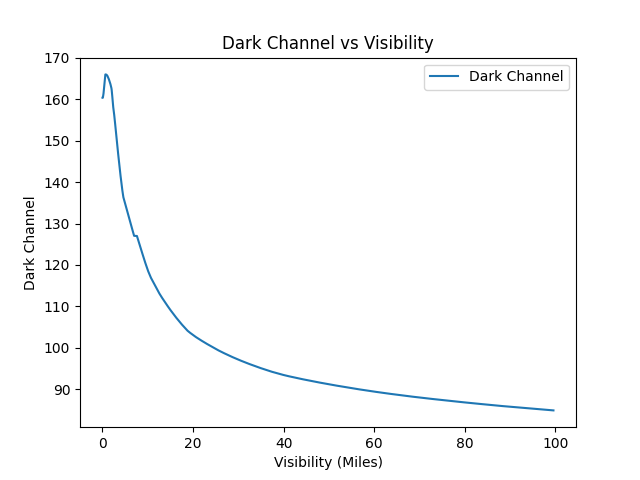
\includegraphics[width=0.2\textwidth]{imgs/dark_channel_vs_visibility.png}} 
%     % Mean of Dark Channel Prior vs Visibility
%     \subfigure[]{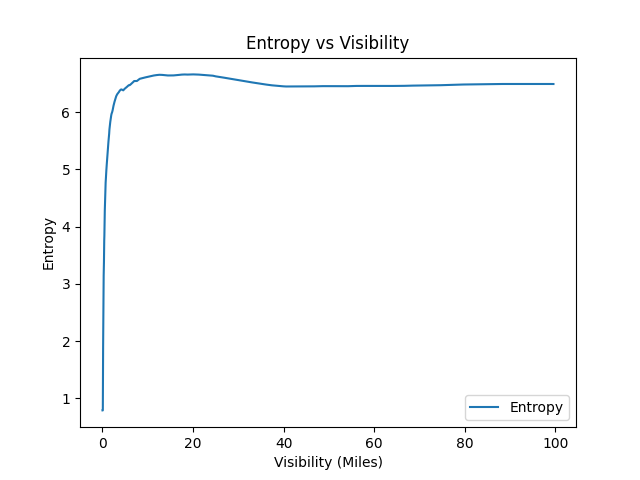
\includegraphics[width=0.2\textwidth]{imgs/entropy_vs_visibility.png}} 
%     % Mean of Edge Density vs Visibility
%     \subfigure[]{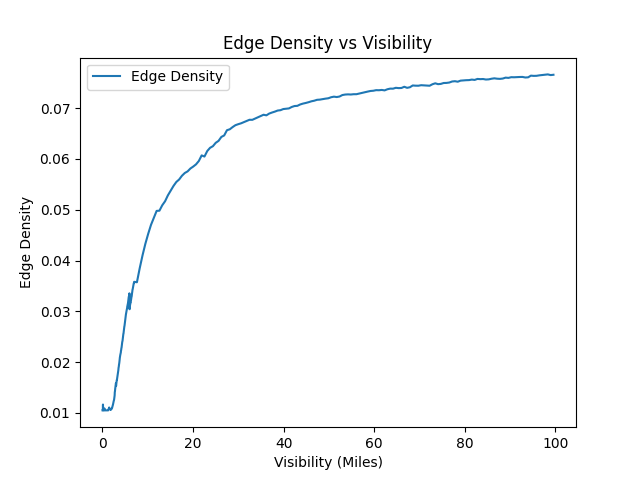
\includegraphics[width=0.2\textwidth]{imgs/edge_density_vs_visibility.png}}
%     % Mean of FFT Magnitude vs Visibility
%     \subfigure[]{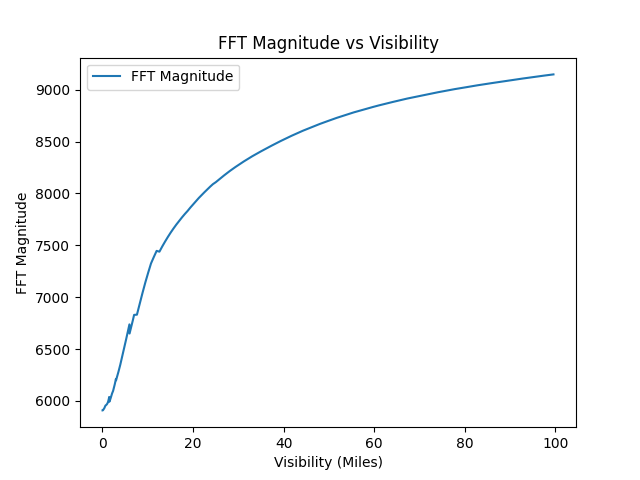
\includegraphics[width=0.2\textwidth]{imgs/fft_magnitude_vs_visibility.png}}
%     \caption{Impact of Visibility Degradation on Edge Density, Entropy, Dark Channel Prior, and FFT Magnitude vs Visibility in Miles}
%     \label{fig:mean_of_features}
% \end{figure*}

 In Figure~\ref{fig:impact_vis_deg_features, fig:mean_of_features}, we show the impact of visibility degradation on various modalities of the same scenery. Each row shows one modality, while each column refers to a visibility bin.